\clearpage
\begingroup
\renewcommand{\thesubsection}{S\arabic{subsection}}
\setcounter{subsection}{0}
\section*{Supplementary Results}

\subsection{International concentration across data sources}
\label{supp:international_sources}

For the fixed set of 203 countries observed throughout the study period, HHI declined from 0.10157 in 1998 to 0.07010 in 2025, compared with 0.10156 to 0.07002 across all countries with flows each year. When every year was sampled at 154,323 international events, HHI declined from 0.10156 to 0.07004 and Gini from 0.9022 to 0.8530.

We recalculated HHI of global national flow shares from the public aggregate origin--destination data accompanying Zhao et al. (2023)\cite{ref039}. This differs from the original paper's country-specific migration-spread measure. After aligning geographic units and removing flows within aggregated units, we selected the same 181 countries with positive combined flow in both sources in each of the four periods: 1998--2002, 2003--2007, 2008--2012 and 2013--2017. Full-network country inflows and outflows were pooled within each period, selected and renormalized before HHI was calculated. HHI declined from 0.10024 to 0.07804 in our data and from 0.08340 to 0.06227 in the Zhao comparator, reductions of 22.14\% and 25.33\%, respectively. Supplementary Fig.~\ref{fig:supp_zhao_hhi} indexes each series to its own first-period HHI. The matched pool retained at least 99.76\% of combined country strength in our data and 99.98\% in the comparator across periods. The published OD table reproduced the author's separate national inflow and outflow totals before geographic alignment. Alignment removed within-unit flow weights of 275, 517, 1,011 and 1,523 across the four periods. These descriptive results show declining concentration in both sources, with a larger relative decline in the comparator.

We also reconstructed an annual comparator from the Scopus-based international flow data accompanying Yenilmez (2026)\cite{yenilmez2026}. This comparison used 1998--2023 and the same 147 countries with positive combined flows in every year in both sources. Geographic units were aligned before full-network country margins were selected and renormalized within this pool. Annual HHI slopes were $-0.00154$ in our series and $-0.00161$ in the comparator. Annual Gini declines were 0.310 and 0.296 percentage points, respectively. The annual HHI series are shown in Supplementary Fig.~\ref{fig:supp_international_hhi}. Endpoint HHI reductions were 32.91\% and 41.64\%; Gini reductions were 8.17\% and 7.90\%. Both sources showed deconcentration, while their relative pace depended on the index. Database coverage and migration-event identification remain source-specific in both comparisons.

\subsection{City-composition accounting}
\label{supp:city_entry}

For each country-year, continuously recorded cities C, intermittently recorded initial cities I, and cities first recorded after 1998 E partitioned the active city set A. Cities in I and E were included only when active. We retained their observed full-network strengths and renormalized each selected distribution. Write F(S) for an index on C plus the groups in S. The entry and intermittent components were
\begin{align*}
e_t&=\tfrac12\{[F_t(E)-F_t(\varnothing)]+[F_t(I,E)-F_t(I)]\},\\
i_t&=\tfrac12\{[F_t(I)-F_t(\varnothing)]+[F_t(I,E)-F_t(E)]\}.
\end{align*}
Thus $M(A_t)=M(C_t)+e_t+i_t$ for each index and country-year. Using the same 28 years, OLS trend slopes also satisfy $b_A=b_C+b_e+b_i$. Additivity was checked at country level, before any summaries across countries. The full and C-only Gini and normalized-count slopes reproduced the existing manuscript values to numerical precision.

The entry component had positive Gini and negative normalized-count slopes in 74 of 76 countries, including 62 of the 63 with observed concentration. It was the largest positive Gini component in 57 of those 63. Across all 76 countries, median Gini trends were +0.244 percentage points per year for all cities, $-0.122$ within C, 0.000 for the intermittent component and +0.373 for entry. These medians are not additive. The median normalized-count entry contribution was $-0.380$ percentage points per year. Entry's HHI component declined in 74 countries, alongside the increases in Gini and declines in the normalized equivalent city count attributable to newly recorded cities. This accounting changes the set of locations in the distribution; it does not simulate how actual flows would respond if cities had not entered.

\subsection{Equal-event sampling and comparative context}
\label{supp:rarefaction}

The primary equal-event analysis used 200 repetitions and seed 20261048. The count of countries with positive Gini and negative normalized-count trends decreased from 63 to 18; positive coverage trends persisted in 72 countries. The minimum annual event total varied by country, with a median of 77.5 events in the full 76-country sample. The 19-country subset with at least 1,000 events in every year was retained as a volume sensitivity analysis in the saved outputs. Equal recorded counts standardize volume but do not remove all differences in publication coverage or city visibility.

Domestic network expansion complements evidence of growing intercity scientific collaboration\cite{ref016}. The all-city Gini increase differs in direction from publication-output deconcentration\cite{ref015} and declining inequality in population-based internal migration rates across regions\cite{ref029}. These studies measure publication counts, population-based regional rates and city flow shares, respectively. These comparisons provide context rather than identify the city-entry contribution.

\subsection{Matched-city disciplinary comparison}
\label{supp:domain_cities}

The primary domestic disciplinary comparison uses the same 45 countries. For the matched-city extension, 34 had at least two cities with positive combined strength in all 28 years in every domain. Each country's same city list was then used in physical, life, health and social sciences. Within these same countries, median Gini slopes changed from positive with annual full city sets to negative with fixed lists in every domain (Supplementary Table~\ref{tab:domain_fixed_city}). The fixed-city subset retains full-network city margins, rather than only links between listed cities. This exploratory extension shows that the primary contrast depends on city membership. It does not identify an intrinsic disciplinary cause.

The primary ranking concerns geographic-distribution change, whereas prior comparisons of individual international mobility rates place physical sciences highest and social sciences lowest\cite{ref033}. Frequency of mobility and the geographic distribution of recorded flows therefore measure different dimensions.
\clearpage
\section*{Supplementary Figures}
\renewcommand{\thefigure}{S\arabic{figure}}
\setcounter{figure}{0}
\begin{figure}[!htbp]
\centering
\makebox[\linewidth][c]{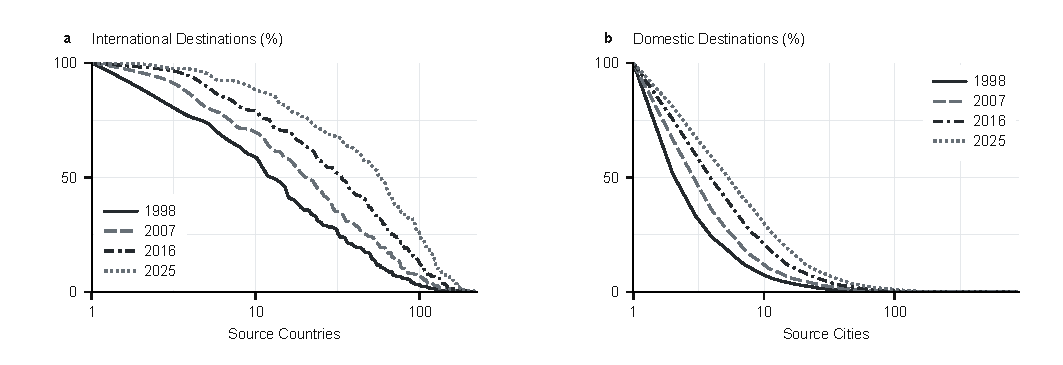
\includegraphics[width=180mm]{figures/FigS1.pdf}}
\caption{\textbar\ \textbf{Expansion in destination reach.} \textbf{a,} Percentages of destination countries connected to at least the indicated number of source countries. \textbf{b,} Percentages of destination cities connected to at least the indicated number of source cities, averaged equally across the 76-country sample. Curves show 1998, 2007, 2016 and 2025, distinguished by line styles.}
\label{fig:supp_coverage}
\end{figure}
\begin{figure}[!htbp]
\centering
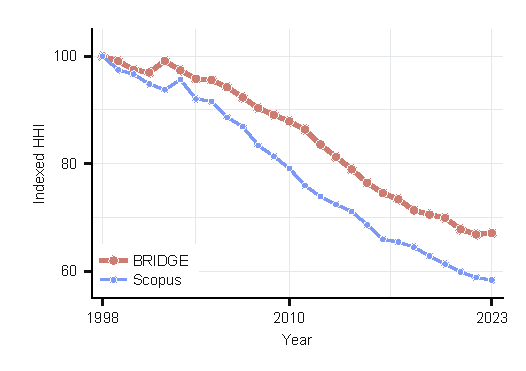
\includegraphics[width=89mm]{figures/FigS2.pdf}
\caption{\textbar\ \textbf{International HHI trajectories across data sources.} Annual HHI in this study (red line, circles) and the Scopus-based data accompanying Yenilmez (2026; blue line, circles)\cite{yenilmez2026}, recalculated over the same 147-country pool for 1998--2023. Each series is indexed to its own 1998 value (1998 = 100). Points show all annual observations and lines connect adjacent years. Geographic units were aligned before full-network country margins were selected and renormalized within the common pool.}
\label{fig:supp_international_hhi}
\end{figure}
\begin{figure}[!htbp]
\centering
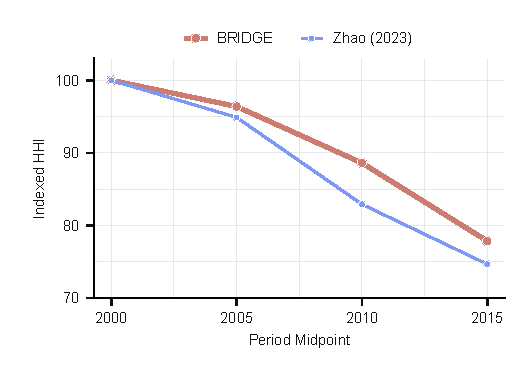
\includegraphics[width=89mm]{figures/FigS3.pdf}
\caption{\textbar\ \textbf{International HHI across matched five-year periods.} HHI of national shares in this study (red) and recalculated from the public Scopus-based flows accompanying Zhao et al. (2023, blue)\cite{ref039}, using the same 181 countries. Flows were pooled within 1998--2002, 2003--2007, 2008--2012 and 2013--2017. Each series is indexed to its own first-period HHI (1998--2002 = 100). Points are positioned at the period midpoints.}
\label{fig:supp_zhao_hhi}
\end{figure}
\FloatBarrier
\endgroup
